\documentclass{article}

\usepackage[utf8]{inputenc}
\usepackage{longtable}
\usepackage{graphicx}
\usepackage[dvipsnames]{xcolor}
\usepackage{enumitem}
\usepackage{xparse}

\title{Cloudy Notes}
\author{Alessandro Biagiotti}
\date{March 2023}

% Definition of enumeration command for rules
\newcounter{descriptcount}

\NewDocumentEnvironment{enumReq}{O{}}{%
    \setcounter{descriptcount}{0}%
    \renewcommand*\descriptionlabel{%
      \stepcounter{descriptcount}%
      \normalfont [R\arabic{descriptcount}]%
    }%
    \description%
  }%
{\enddescription}

\begin{document}

\maketitle

% Command definitions
\newcommand{\subSkip}{\vspace{1cm}\\}
\newcommand{\smallSkip}{\vspace{0.5cm}\\}
\newcommand{\miniSkip}{\vspace{3pt}\\}
\newcommand{\subSpace}{\vspace{1cm}}
\newcommand{\smallSpace}{\vspace{0.5cm}}
\newcommand{\miniSpace}{\vspace{3pt}}
\newcommand{\n}{\\}
\newcommand{\pink}[1]{{\color{WildStrawberry} #1} }
\newcommand{\elt}{\pink{ELT}}
\newcommand{\lb}[1]{{\color{ProcessBlue} #1} }
\newcommand{\etl}{\lb{ETL}}

\tableofcontents
\clearpage

% Chapters
\section{Introduction}
First, we want to focus on the concept of a distributed system, which is, intuitively, a complex mechanism with many moving parts. The parts can move on their own or according to the plans of a master that is keeping everything under control. We will see a couple of different definitions that try to encapsulate what distributed systems are all about. \\
A distributed system can be seen as two or more computers, each one with its own local memory and processor, connected via networking communication. \\
Basically this means that a distributed system is none other than a group of computer communicating via the exchange of messages. \\
Distribution can be at three different levels:
\begin{itemize}
    \item Hardware
    \item Data, which, to be processed, needs to be replicated and partitioned
    \item Control
\end{itemize}
What is the difference between centralized and distributed systems? \\
\begin{table}[h!]
    \centering
    \begin{tabular}{| c | c |}
        \hline
        \multicolumn{2}{| c |}{Differences}\\ 
        \hline
        Distributed & Centralized\\
        \hline
        Autonomous components & Non autonomous components\\
        \hline
        Heterogeneous technology & Most of the time build using homogeneous technology\\
        \hline
        Components can be used exclusively & multiple users share the same resources all times\\
        \hline
        Executed in concurrent processes & single point of control and of failure\\
        \hline
        Multiple points of failure & ;D\\
        \hline
    \end{tabular}
\end{table}
An important question needs to find an answer, why do we bother with distributed systems? Is the added complexity really beneficial? \\
The answer is, obviously, yes (to some extent). 
\begin{itemize}
    \item Distributed systems allow for functional separation between the agents in action.
    \item The model goes toe to toe with the conception of information we have today.
    \item We can distribute computational load over many devices instead of having only one node to complete the task. This is really beneficial for complex tasks.
    \item Distributed systems are very reliable
    \item Sharing a pool of resources with many individuals make them very economical because we don't need to buy many for each one, we just need many resources for many people.
\end{itemize}
Another good definition of a distributed system is the following:
\begin{center}
    \textit{"A distributed system is a collection of autonomous computing elements that appears to its users as a single coherent system"}
\end{center}
This means that a distributed system is basically a network of very different devices, each with its own hardware, its own os, etc... And it appears as if it was a single and coherent entity. \\
To make this possible we have to mount a middleware layer on top of the operating system of each of the machines, this middleware will filter requests coming from the outside and translate them in something that can be understood by the underlying operating system. The process, although, is completely transparent to the user. \\
To be mor specific, what are the tasks that a middleware should be able to handle?
\begin{itemize}
    \item It should manage resources offering its applications to efficiently share and deploy those resources across a network.
    \item It should offer facilities for inter application communication.
    \item It should handle security.
    \item It should handle accounting services.
    \item It should mask the recovery failures (not trivial).
\end{itemize}
Now, before analyzing some practical examples of distributed systems, let's consider some very important design goals that should be considered when handling these models.
\subsection{Transparency}
Transparency is a very important concept in computer science, just think about how transparency plays a role in object oriented programming, in the field of distributed computing even more so. We would like to have a system that is easy to use and can easily hid what lies on the other side. \\
Unfortunately transparency is very hard to achieve (full trainsparency is even impossible), we ended up defining a series of types of transparency that have different meanings:
\begin{table}[h!]
    \centering
    \begin{tabular}{| c | c |}
        \hline
        \multicolumn{2}{| c |}{Some types of transparency}\\ 
        \hline
        Transparency & Description\\
        \hline
        Access & Hide differences in data representation and how an object is accessed\\
        \hline
        Location & Hide where an objects is located\\
        \hline
        Relocation & Hide that an object may move to another location\\
        \hline
        Replication & Hide that an object is replicated\\
        \hline
        Concurrency & Hide that an object may be shared by several independent users\\
        \hline
        Failure & Hide the failure and recover of an object\\
        \hline
    \end{tabular}
\end{table}
Needless to say that having so many moving parts while trying to hide one or more of the above details can make programming and debugging a distributed system a very complex process. \\
\subsection{Openness and Scalability}
A distributed (or operating) system is open when anybody is able to make modifications to the modules that compose it, here is very important to stress a point. Rendering a distributed system open doesn't mean handing all of your personal code over to people, you are just required to make it so that anyone can make modifications without touching the core logic. This is the logic of separating the policy from the mechanism. \\
A silly example can be: If I produced some kind of remote communication service that uses certain protocols, anyone should be able to choose another protocol to work with and attatch his own code to mine so that it all works seamlessly. \\
A distributed system should always be scalable, there are three different ways to scale a system:
\begin{itemize}
    \item Scale in size (number of users or/and processes)
    \item Geographical Scalability
    \item Administrative domanis: The system spans multiple administrative domains
\end{itemize}
When scaling is needed we can either scale up, by basically improving the singular hardware specs of the various machines, or scale out, by expanding the fleet of machines that compose the distributed system. \\
One of the classical problems of scaling out is the replication issue, where we have multiple copies of the same file over many machines in the network. This has a series of effects, first and foremost inconsistency, we usually have to keep track of whichever is the most up to date version of the file. Secondly we have to decide how to handle them, because inconsistencies will surely be present. We can either, as an example, update all of the various copies of the file whenever it changes, or we can keep different versions of the file in the network and, whenever prompted, look for the most up to date currently available.
\subSpace
The following are a series of false assumptions that developers tend to make when modelling a distributed system:
\begin{itemize}
    \item The network is reliable.
    \item The network is secure.
    \item The network is homogeneous.
    \item The topology does not change.
    \item Latency is zero.
    \item Bandwidth is infinite.
    \item Transport cost is zero.
    \item One single administrator.
\end{itemize}
\subsection{Types of distributed systems}
We will now explore two different models for distributed systems.
\subsubsection{High performance distributed computing}
High performance distirbuted computing is a very cool field to explore because it's the founding idea of current supercomputers, which dispose of various computing modules that are employed based on the type of load that is hitting the system. \\
We usually talk about Cluster computing, in which we have similar workstations connected to a high-speed network, each machine is running the same os, or Grid Computing, which is an heterogeneous network of machines dispersed across several organ. \\
Cloud computing is another technique for high performance distributed computing, but it's meant for prosumer use and that is because a cloud workstation can be bought for relatively cheap, employed right away and extended at the client's leisure.
\subsubsection{Distributed information systems}
Distributed information systems allow for resilient backup of data. This model is based on the concept of transaction, which is an event that involves a client and a server, for the transaction to take place everything needs to go according to plan (just like an economical transaction). \\
Transactions must follow the ACID properties:
\begin{itemize}
    \item Atomic: The transaction must be indivisible.
    \item Consistent: The transaction must not violate system invariants.
    \item Isolated: Concurrent transactions do not interfere with each other.
    \item Durable: Once a transaction commits, changes are permanent.
\end{itemize}
Usually transactions are constructed as a group of subtransactions that run in parallel. This division provides a natural way of distributing a transaction across multiple machines.
\subsubsection{Pervasive systems}
Pervasive systems are networks composed of nodes that are often small, mobile and embedded in larger systems, characterized by the fact that the system naturally blends into the user's environment. In the field of pervasive systems we have three different categories:
\begin{itemize}
    \item Ubiquitous computing: Pervasive and continuously present
    \item Mobile computing: Pervasive but inherently mobile
    \item Sensor networks
\end{itemize}
\textbf{Uniquitous computing} \\
The core requirements for Ubiquitous computing systems are the following:
\begin{itemize}
    \item Distribution: The device and network are accessible in a transparent manner (even though they are distributed).
    \item Interaction: The system is highly unobtrusive.
    \item Context awareness: To optimize the interaction the system is aware of a user's context.
    \item Autonomy: Devices must be autonomous.
    \item The system can handle a wide range of dynamic actions and interactions.
\end{itemize}
\textbf{Mobile computing} \\
A distributed system in which there are many different devices with very different architectures, all connected via wireless and in movement. Since the setting for the connection is really complex it's essentially a disruption-tolerant network. \\
\textbf{Sensor network} \\
A sensor network should be a network of many sensors implied in different scenarios (the first that comes to mind is a Nuclear implant sensor network), the devices themselves are very simple. Essentially this kind of sensor network is organized as a distributed database, sensors send data to the operator, store data and respond to queries.
The nodes have very low amount of memory and low computing capabilities, they store just enough to make simple computations and the rest is left to a more capable node in the network. We can think about a more centralized architecture (aka the nuclear implant above) or a more distributed scenario (IoT).
\section{Architectures}
Software architectures show the logical organizazion of a distributed system into software components, the system architecture is the final instantiation of the theoretical software architecture. \n
A couple of well known architectural styles are:
\begin{itemize}
    \item Layered
    \item Object oriented
    \item Resource orienteted
    \item Event based
\end{itemize}
Now we'll rapidly go through each of them. \n
\textbf{Layered architecture} \n
Components are organized in a layered fashion, a component can make a downcall (as in the case of calls to the operating system). \n
Upcalls are exceptions.
\smallSpace
\textbf{Object oriented architecture} \n
The components in an object oriented architecture are objects and connect to each other through procedure calls, the calls can be distributed if the objects are on different machines. \n
In the distributed case we can have separation of interfaces and objects and we can do calls via RPC. \n
Service oriented architectures are distributed applications constructed via service composition. \n
\smallSpace
\textbf{Resource base architectures} \n
A REST architecture is focused on resources and their indexing. Usually we have an interface that exposes a series of methods concerning actions we can do with respect to them. In a REST architecture:
\begin{itemize}
    \item Resources are identified through a single naming scheme
    \item All services offer the same interface
    \item Messages sent to or from service are fully self-described
    \item The communication is stateless
    \item The operations we can do with resources are a few and are standard.
\end{itemize}
When building a software architecture we are in front of two very different structures. Centralized organization, in which we have a server offering and a client recieving, the communication is of type request reply. \n
An example of centralized organization is a multitiered architecture, in which we have a client and one or more servers handling different aspects of the service (as an example: the MVC architecture, where we have a division between Model (data), View (frontend), Control (backend)). \n
When working with a multitiered architecture we can use two different models:
\begin{itemize}
    \item Vertical distribution: We divide the distributed applciation into three logical layers and we run the components from each layer on a different server.
    \item Horizontal distribution: A client or server can be physically split up into logically equivalent parts. Each part is operating on its own share of the complete data set (balancing the load).
\end{itemize}
The opposite of Centralized architecture is the Decentralized architecture, which are peer-to-peer architectures. \n
In peer-to-peer systems each node of the network is considered on the same level of the others, each of them can access data possessed by other nodes in the network and share its own. Not all peer-to-peer are built the same, it can be:
\begin{itemize}
    \item Structured: it's an overlay that adheres to a specific topology and uses a semantic-free index where each data item is uniquely associated with a key. For lookup we use a distributed hastable.
    \item Unstructured: In which we have an ad-hoc list of neighbours, to search data we can either flood the network or do a random walk.
    \item Hierarchically organized: We have a super peer which acts like an orchestrator, an index server and brokers to decide where to store data. An example of this is a Content Delivery Network.
\end{itemize}
Like with everything it's not always either black or white, we have hybrid architectures in which we combine a decentralized architecture with the client-server archetipe. \n
An example of hybrid architecture is the \textbf{Edge-server architecture} which uses client-server to manage the connection between private networks placed outside of internet's bounds and use an orchestrator or an edge server to communicate with the world. \n
Another example are collaborative distributed systems like Emule, bitTorrent, et al...
\begin{figure}[htb]
    \centering
    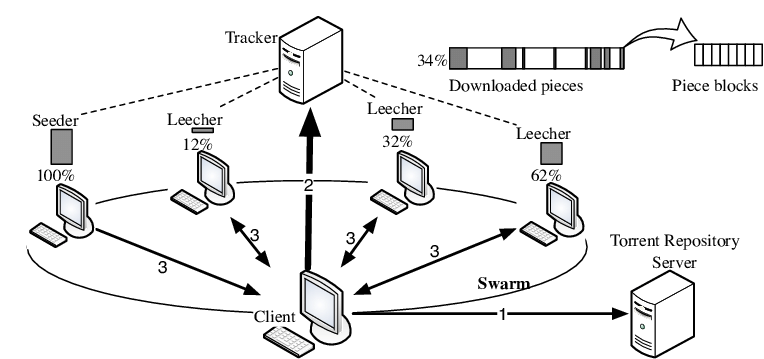
\includegraphics[scale=0.45]{./Images/bittorrent.png}
    \caption{Structure of the bitTorrent network}
\end{figure}

\section{Processes}
Now we will go through a very fast review of what processes and light processes are, first and foremost a very basic, but important, distinction needs to be made between a series of concepts.
The \textbf{Processor} is the hardware that is used to process instructions coming from programs, a \textbf{Thread} (also known as light process) is a minimal software processor in whose context a series of instructions can be executed; finally, the \textbf{Process}, is a software processor in whose context one or more Threads can be executed. \n
Why do we have two different types of processes? Not everyone knows that context switching, the operation of changing the contents of the registers in the Processor, is very heavy and it's done every single time we switch Processes during the computation. Using threads is much easier because it allows us to parallelize computation within the same process and they share the address space for memory access. \n
Basically having Threads allows us to: avoid waits when doing I/O operations, take advantage of multiprocessor architectures by parallelizing operations and avoid process switching in the context of a single large application. \n
The trade off is that we need to be aware of the fact that programming for parallallelized environment is complex from many points of view. A very classical example of multithreading is in the client-server communiucation, where the server can be multithreaded to handle multiple requests at the same time and avoiding that some slower one prevents the process from working correctly. \n
\section{Virtualization}
Virtualization is a concept which is closely related to the one of Processes and multithreading, virtualization deals with extending or replacing an existing interface mimicing the behaviour of another system. \\
Virtualization is, nowadays, a standard; that is because it allows to handle hardware changes with ease because the hardware is virtualized and the interface does not change for the above system. With virtualization also come ease of portability and code migration and isolation of failing or attacked components. \\
There are different ways to do virtualization, a couple of interfaces to be virtualized are the following:
\begin{itemize}
    \item Instruction set architecture
    \item System calls
    \item Library calls
    \item Process virtualization in which we have a separate set of instructions, an interpreter/emulator, running atop an OS
    \item Native virtual machine monitor in which we have low level instructions along with barebones minimal operating system
    \item Hosted virtual machine monitor in which we have low level instructions but most of the work is delegated to a full fladged OS.
\end{itemize}
Now we will talk about virtualization and everything that revolves around it more in detail. \\
First virtualization is an activity aiming to create replacements for real resources, which have the same functionalities and external interfaces of their counterpart, but different attributes. \\
The concept of emulation and simulation are linked to virtualization, the three concepts mean different things. \\
\begin{itemize}
    \item Emulation: We execute a system like it is another system. We run os, API and functions on a machine which they have not been developed for.
    \item Simulation: An application allowing to execute old programs defined for different platforms on modern machines and it replicates the behaviour of a system. It's like a software emulation. \\
    Emulation is slower but precise while simulation is fast but less precise. We use simulation (or software emulation, to run old games on our smartphones).
    \item High level emulation is an intermediate between emulation and simulation, they recreate the functionalities of an emulated system using similar or equivalent functions in the emulating system.
    \item Virtualization: the technique for using resources and devices in a functional way without considering their physical layout. \\
    In the world of virtualization a Virtual Machine is a container with software based CPU, RAM and HDD and network connection. We have a certain level of transparency because an OS or an application do not distinguish between a virtual and a physical machine.
\end{itemize}
\begin{figure}
    \centering
    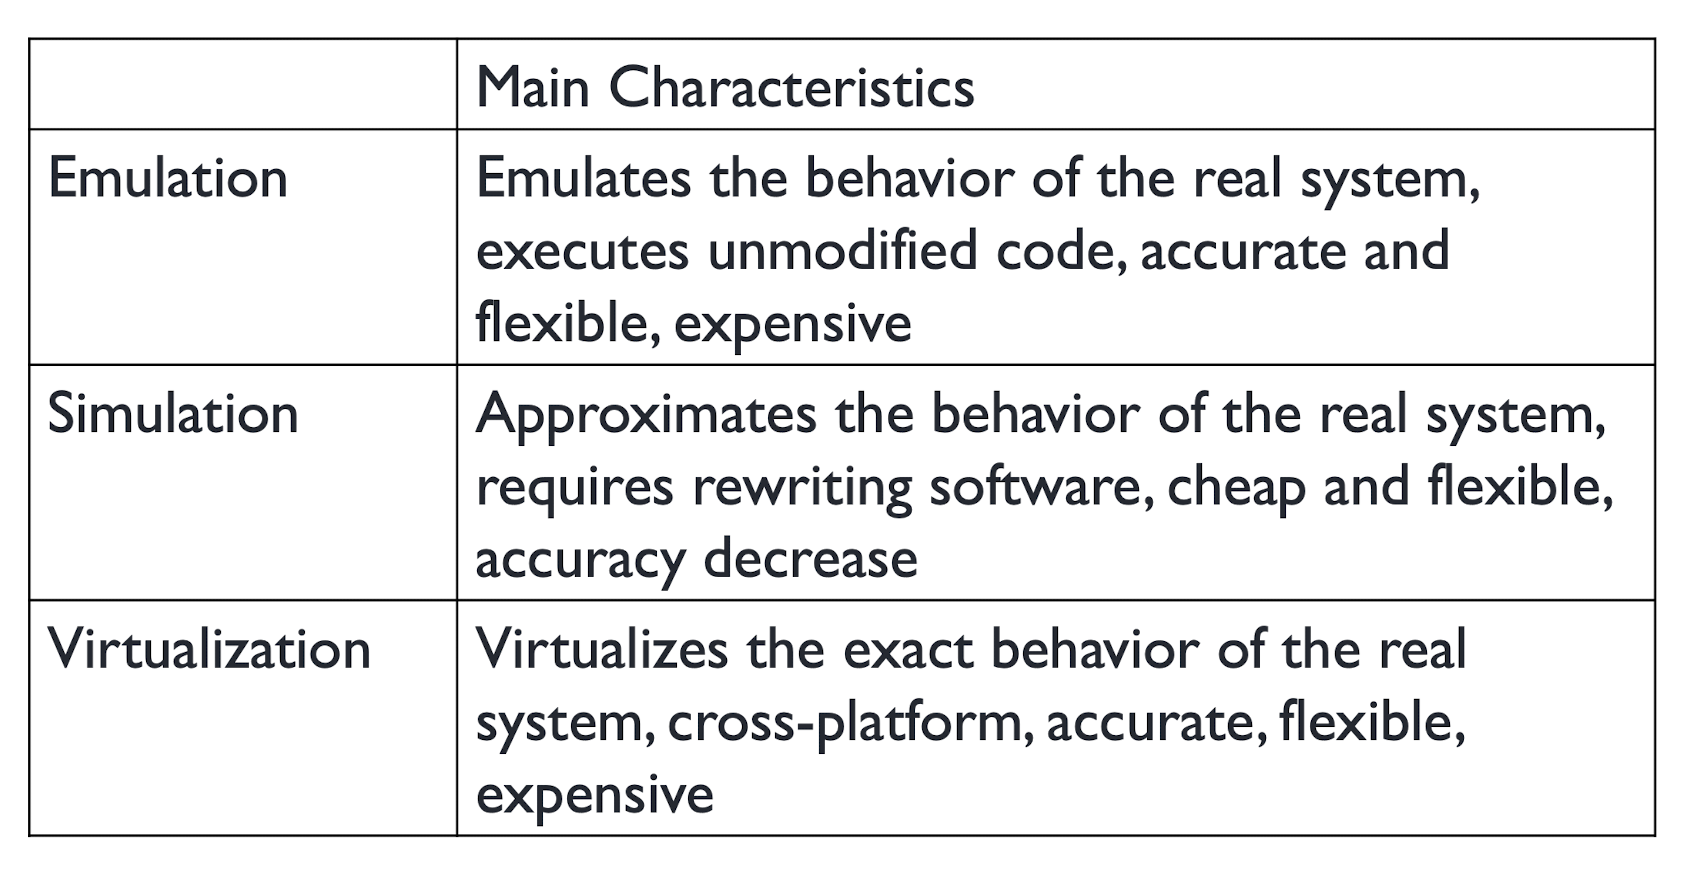
\includegraphics[scale=0.4]{./Images/summary_virtualization.png}
    \caption{Summary of the principal characteristics of virtualization techniques}
\end{figure}
Now we will focus on each one separately.
\subsection{Virtualization}
Virtualization is compatible with x86/64 machines, each has a full and dedicated environment and each machine is isolated from each other just like physical separation. \\
Virtualization was created to solve some issues:
\begin{itemize}
    \item Too many servers but small workloads
    \item Old hardware does not work
    \item Infrastructural requirements are always increasing (many independent servers)
    \item Small flexibility in shared environments
\end{itemize}
Virtualization allows to keep the costs low for resources while managing them efficiently and keeping the necessary computational power. We can, in fact, use a single hardware server as a multitude of virtual servers. \\
If a cloud solution has been deployed well we can use virtualization to increase resource usage and enable dynamic sharing of resource pools. We can even react to particular situations because virtualization allows us to have a single consolidated view of each resource of the network which can be easily accessed, moved and managed from wherever. \\
Other reasons that support the choice of going virtualized are the following:
\begin{itemize}
    \item Better performance
    \item transparency
    \item Heterogeneity
    \item portability
    \item Interoperability
    \item Green IT (with the same amount of hardware we satisfy more people)
\end{itemize}
Virtualization can be used in many different scenarios, it's heavily used in cloud-based applications because we can, for example, virtualize resources into pools and assign them to users based on the fee they pay and on their workload. \\
We can also use virtualization to deploy microservice-based applications by putting every microservice into its own virtualized container. \\
As a last example we can use virtualization to keep our systems secure, with a virtualized environment we can test code and / or applications to see that they work / do not contain viruses before downloading them on our own machine. \\
A couple of reasons against virtualization are the follwing:
\begin{itemize}
    \item Analysis and planning: building an application or a service that stands on top of a virtualized environment is easy enough, porting something to a virtualized environment a completely different workflow. A lot of planning and study has to go into the process, the staff needs to be trained and a lot of risk analysis has to be done.
    \item Adaptation and post adaptation: A lof of evaluation needs to go into studying the relaiability, the performance, the efficiency and the security of the virtualized environment that will be used.
    \item Maintenance: Maintenance must be kept in mind as well, mostly scalability and security.
\end{itemize}
\begin{figure}
    \centering
    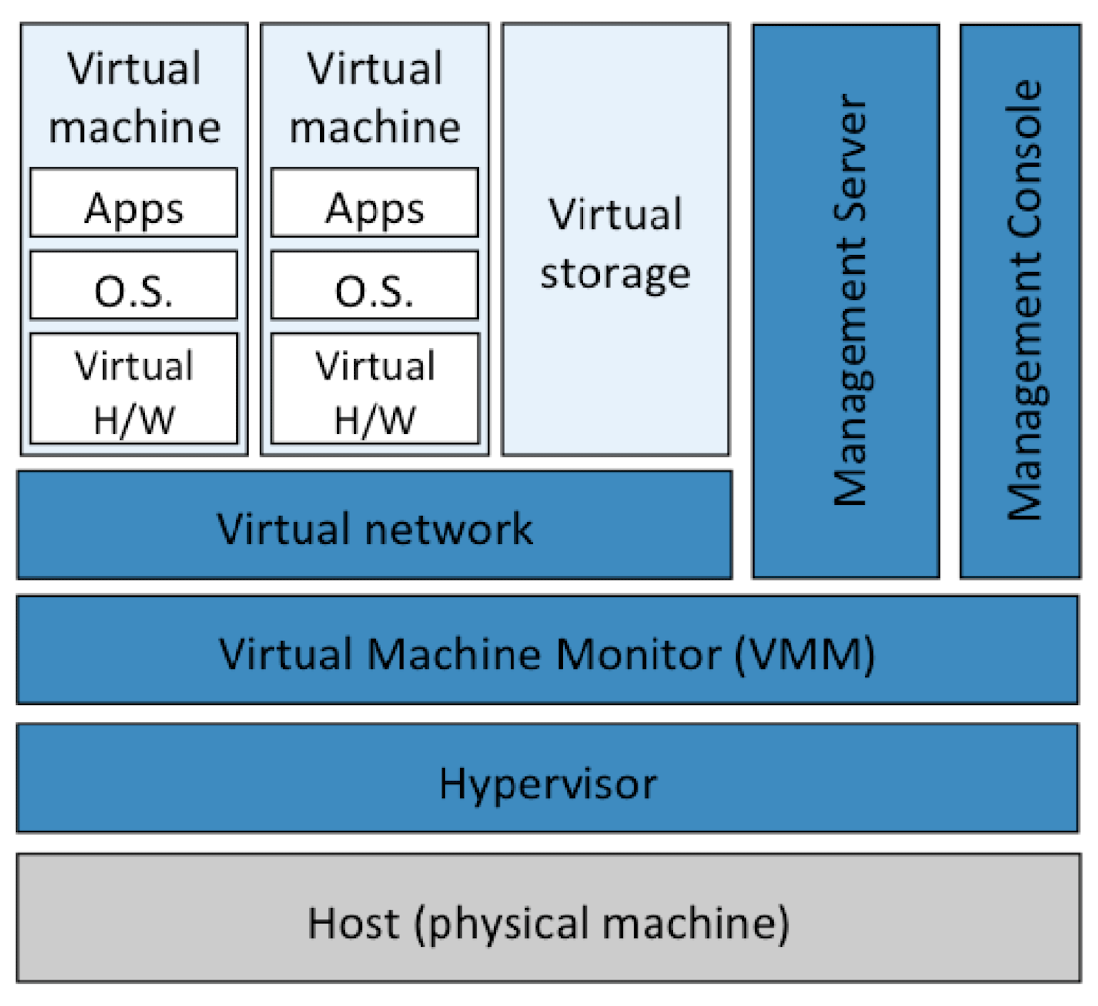
\includegraphics[scale=0.4]{./Images/virtualization_components.png}
    \caption{The structure of a virtualizer}
\end{figure}
Now we'll take a look at the structure of a virtualizer. \\
The components are the following: \\
\smallSpace
\textbf{Hypervisor} \\
The Hypervisor is a component that interacts with the virtual machine and with the host, it allows for multiple OSs running on the same computer. Beware! In the case of an operating system like windows it's important to keep in mind that turning on the Hypervisor and having a virtual machine manager like Virtual Box or VMware may cause instabilities. \\
\smallSpace
\textbf{Virtual machine monitor}\\
It's the application component realizing virtualization. \\
\smallSpace
\textbf{Guest OS} \\
\smallSpace
\textbf{Host OS} \\
\smallSpace
\textbf{management Server} \\
It's a virtualization platform.
\smallSpace
\textbf{Management Console} \\
Provides access to the virtualization management interface. \\
\subSpace
A cool factoid about virtualization is that there is a non-mandatory constraint that requires that a statistically relevant percentage of instructions inside a virtualized environment should be executed without virtualization. Abiding to this rule will guarantee better efficiency of the virtual machine. \\
Now we will consider a couple of different virtualization models. 
\begin{figure}
    \centering
    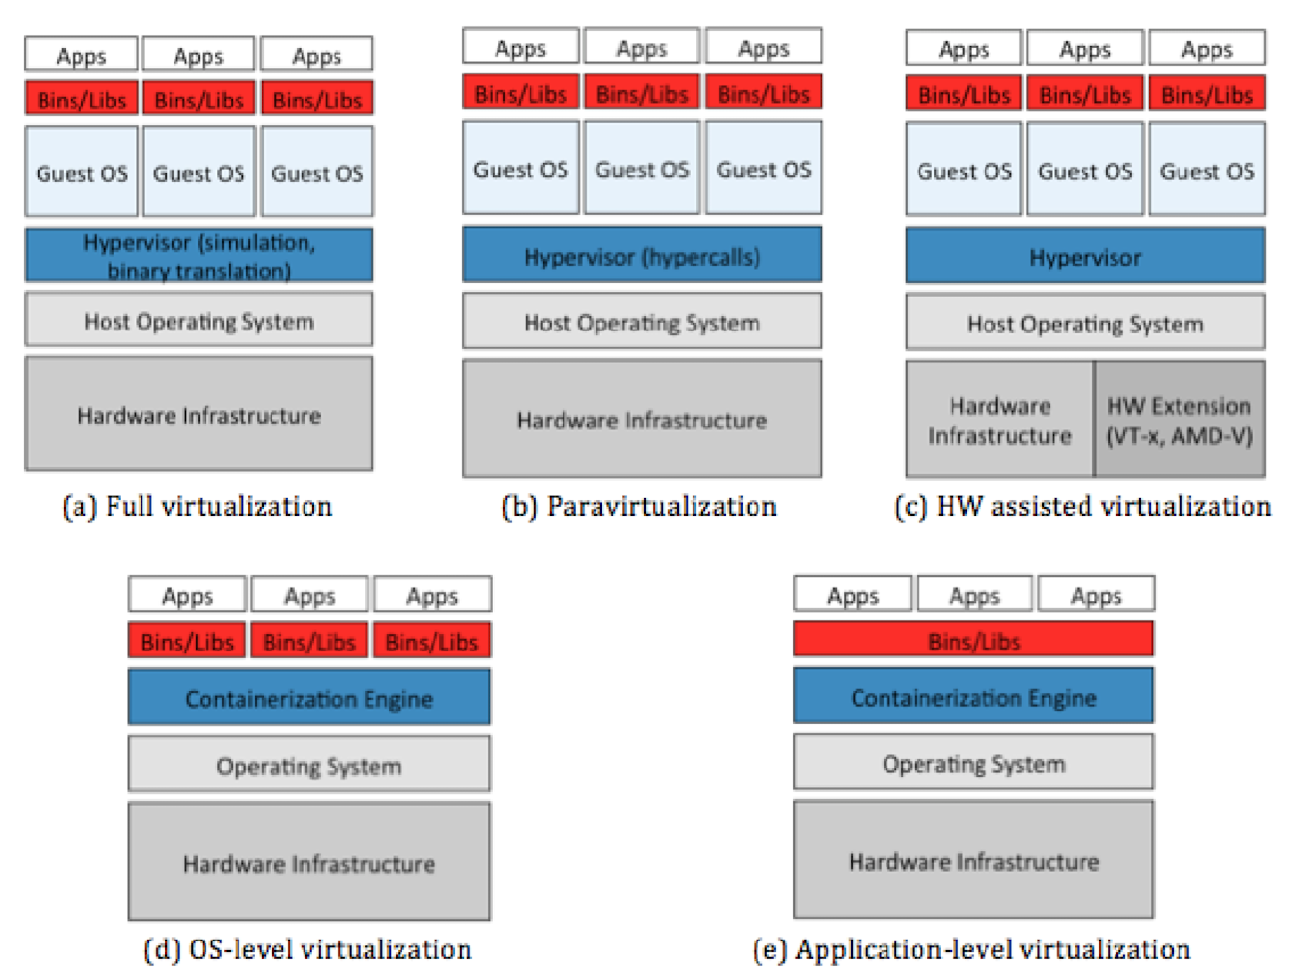
\includegraphics[scale=0.4]{./Images/virtualization_stacks.png}
    \caption{Various virtualization models}
\end{figure}
When doing \textbf{Full emulation}, we emulate every aspect of a computer and it allows to execute an unmodified guest OS on a completely different host architecture. \\
\miniSpace
\textbf{Full virtualization} [4a], instead, only emulates the necessary hardware, allowing the isolated execution of a guest OS, the only difference is that the guest OS must be designed for the same architecture. \\
\miniSpace
If we need to run software for MIPS-32 architecture we are going to need to emulate the whole machine because we cannot run a virtual machine made for something like that on x86. \\
\miniSpace
Nowadays processors come with instructions that allow to provide the virtual machine with some true hardware (\textbf{Hardware assisted virtualization} [4c]). That boosts machine performance with full virtualization. \\
\miniSpace
\textbf{Paravirtualization} [4b] is another form of virtualization where the virtual machine makes available an API to extend the guest OS (the guest OS has to be modified), the extension consists of hypercall implementation which is a virtualized version of a system call. Basically it's a way of opening a direct line of communication between the Guest OS and the Hypervisor below. \\
\miniSpace
In \textbf{OS-level virtualization} [4d] the virtual machine manager partitions hardware resources of host OS between the guests. The host OS guarantees the isolation of multiple user space instances. \\
\miniSpace
In \textbf{Application level virtualization} [4e] we have a virtualized application that runs in a safe and enclosed environment, this avoids risky memory overwrites that may break the operating system. This also allows for better portability of code. \\
\smallSpace
Virtualization can either be native or non-native, if it's native is fast because guest OS and host OS coincide and, probably, the Hypervisor is very low level and very efficient. In the other case we are working with a slower form of virtualization but it allows to have different operating systems. \\

\subsection{Virtualization Software}
Now we will se a couple of specific solutions for hardware virtualization.
\subsubsection{VMware ESXi}
\subsubsection{Xen}
\subsubsection{KVM}
\section{Introduction to Cloud}
In this section we will see the roots of cloud computing, which is a weird brew of different concepts: hardware virtualization, internet technologies, distributed systems and system management. \n
We'll go rapidly through the various concepts needed.
\subsection{Distributed Systems}
We have talked extensively about Distributed systems previously, just as a refresher, a distributed system is an heterogeneous set of N autonomous processors (sites), n administrators, n operating systems, n data/control flows.
\subsection{SOA}
A SOA is a Service Oriented Architecture, it's an open standard for software integrazion and uses a standardized web service software stack. \n
A Service Oriented Architecture implements the concepts of distributed system and computing providing a loosely-coupled, standard and protocol independent system. SOA used a protocol called SOAP that was very complex to use but very descriptive. Service Oriented Architectures aren't all that used anymore in web development because it's much easier to setup REST applications. \n
Cloud applications are developed as service compositions at different layers.
\subsection{Computing models}
There are many different computing models, we'll see a couple of them in the following:
\begin{itemize}
    \item Cluster computing: computers are interconnected through an high performance network and basically form a unique entity.
    \item Network computing: cluster computing extended to WAN.
    \item Meta computing: very old technique for distributed computing.
    \item Grid computing: Coordinated resource sharing and problem solving in a dynamic, multi institutional virtual organizations. \n
    This model relies on Web Service standard protocols.
    \item Utility computing: On demand delivery of infrastructure, applications, and business processes in a security rich, shared, scalable, and standard-based computer environment over the internet for a fee.
    \item Autonomic computing: autonomic systems with self management that provide adaptation mechanisms and reduce user involvement.
\end{itemize}
\subsection{Cloud computing}
Cloud computing is a mashup of some of the previous computing models, in particular autonomic and distributed systems. \n
The idea of cloud computing is to provide IT as a service. Storage, data processing and additional IT services distributed by external providers, applications are computing utilities and users have no need to know how they work beneath. The user pays as he goes depending on the type of service required. \n
As for distributed systems there are many different definitions for cloud computing, the more interesting one is the NIST definition, which follows:
\begin{center}
    \textit{Cloud computing is a model for enabling ubiquitous, convenient, on-demand network access to a shared pool of configurable computing resources that can be rapidly provisioned and released with minimal management effort or service provider interaction. This cloud model is composed of five essential characteristics, three service models, and four deployment models.}
\end{center}
We'll now go through the essential characteristics of cloud computing, if a cloud architecture doesn't implement all of them the architecture will perform bad and won't be used by many people as a result.
\begin{itemize}
    \item On demand, self-service \n
    A client can procure resources, server time and network storage on demand.
    \item Broad network access \n
    Accessing the cloud platform should be easy and should be supported via standard web protocols on any device.
    \item Rapid elasticity \n
    The network should be able to scale out, in and down\footnote{
        The difference between scaling in and scaling down is that scaling in involves adding resources to handle increased demand, while scaling down involves reducing resources as demand decreases.
    } automatically depending on the load. There should be minimal-to-none resource waste.
    \item Measured service \n
    Resource usage is monitored, controlled, and logged providing transparency to cloud providers and customers.
    \item Resource pooling
\end{itemize}
Some additional characteristics are the following
\begin{itemize}
    \item Lower costs
    \item Ease of use
    \item Quality of Service
    \item Reliability
    \item Outsourced IT management
\end{itemize}
A fundamental aspect of cloud computing is Multi-tenancy which means that a aingle software instance is shared by different enterprises/clients (tenants). Data, via virtualization, is isolated but we have no physical isolation. \n
The pros of multi-tenancy are that the cloud provider pays less for hardware and he can provide dynamic access to shared resources. \n
The cons are that users might access data of other users and data backup and data restore are more difficult.
\subsection{Infrastructure as a Service}
Users manage the whole machine, they have virtualized hardware resources associated to them and can install basically anything on the machines as if they had a box next to them. The user has a limited control of network components. \n
Companies provide different servers with different operating systems and an ad hoc stack software, Amazon offers virtual machines with tifferent combinations of operating systems. \n
The advantages of IaaS are:
\begin{itemize}
    \item Pay per use
    \item Modular scalability
    \item Sercurity
    \item Reliability
    \item APIs
\end{itemize}
An example can be having a virtual machine with Linux and using it via the network to handle an heavy compilation process.
\subsection{Platform as a Service}
Users install and create applications developed using programming languages, libraries, services and tools supported by the provider. \n
An example of PaaS is ReplIT which is a platform for coding, compiling and running code. The difference between PaaS and IaaS is that in the first case the user has no control over the system below, the provider offers a complete package for a certain type of development and basically nothing underneath can be changed. \n
The advantages of PaaS are the same as above.
\subsection{Software as a Service}
In the SaaS model users can use applications executed on the cloud infrastructure, users do not manage or control the cloud infrastructre and application-specific functionalities. Users can only control a limited number of user-specific configurations.
\subsection{Cloud stack and deployment models}
Every XaaS in the stack has a couple of common characteristics:
\begin{itemize}
    \item Low costs of maintenance
    \item Management of peaks of traffic
    \item Fast application roll-out
\end{itemize}
\begin{figure}
    \centering
    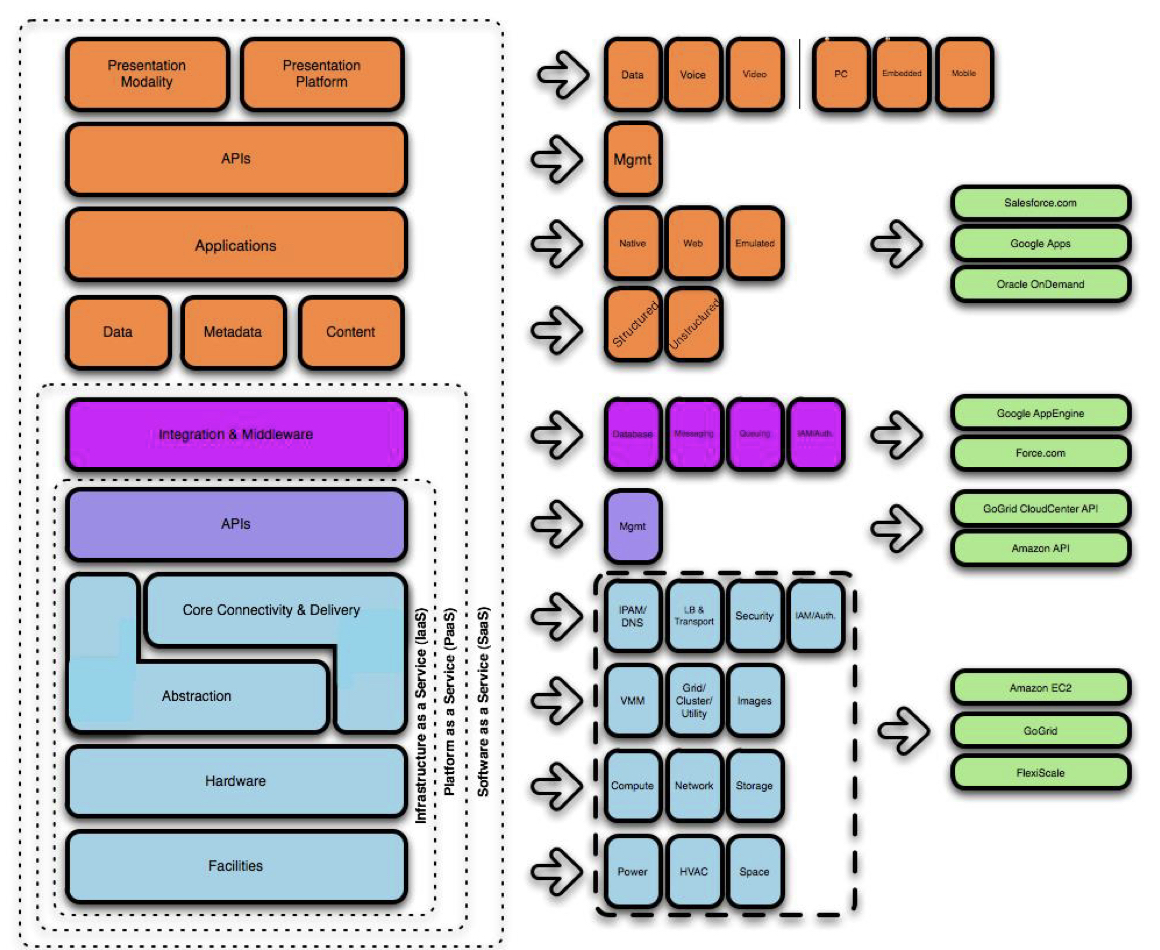
\includegraphics[scale=0.2]{./Images/cloud_stack.jpeg}
    \caption{The cloud stack, every layer of the XaaS stack is built on top of the services of the layer below}
\end{figure}
Cloud services can be deployed in a couple of different ways depending on who should have access to the services. \n
If the cloud infrastructure is provided exclusively for a single organization including multiple tenants, an example of private clud is the machine we can access via the cloud at SiLab in Unimi. The cloud infrastructure is owned and managed by a single organization (the solution can either be private or third party thus can be on premise or off premise). \n
If the cloud infrastructure is provided for an exclusive use of a community of users and is owned and managed by one or more organizations, thrd parties or a combination of the two we are talking about Community cloud. \n
If the cloud infrastructure is public we are talking about Public Cloud, an example of public cloud is OneDrive. \n
If the cloud infrastructure is a combination of two or more cloud infrastructures we are talking about Hybrid Cloud, each infrastructure remains separated, but are composed using standard or proprietary technologies. \n
\section{Migration and cloudonomics}
Even though the course is about cloud computing like any business solution it's not the only one, before choosing which route to take we should make sure to understand:
\begin{itemize}
    \item Where is headed our business?
    \item What are we trying to achieve?
    \item Which are the goals of our business?
\end{itemize}
The replies to these questions give an end goal, with an end goal we can understand what kind of technologies we should be using.
\subsection{Cloud Migration}
Now we'll concentrate on the concept of migration, when should we consider migration to the cloud? Which part of an IT application must or can be migrated to the cloud? Which does not? \n
Let's recall why cloud is considered to be a good solution. It will reduce complexity of system management and will allow to scale easily in order to accomodate more users. \n
What does cloud computing promise?
\begin{itemize}
    \item Full network reliability.
    \item Zero network latency.
    \item Infinite bandwidth.
    \item Secure network.
    \item No topology change.
    \item Centralized administration.
    \item Zero transport cost.
    \item Homogeneous netwrok and system.
    \item Security.
    \item Performance monitoring.
    \item Consistend and robust service abstraction.
    \item Meta scheduling.
    \item Energy-efficient load balancing.
    \item Scale management.
    \item SLA \& QoS architectures.
    \item Interoperability and portability.
    \item Green IT.
\end{itemize}
A company should migrate to cloud because it's going to cost them less than having hardware and software working on premise and it will allow them to scale easily depending on the amount of people that use their services. \n 
The cloud solution allows the company to concentrate on the service they want to offer and forget about the underlying infrastructure. Now we will take a look at the differences between going cloud and offering the same on premise.
\subsubsection{On demand resourcing}
Adding additional resources to a datacenter on premise is really can be really difficult and challenging, if the servers are "on fire" the company can get new hardware but the process of obtaining new hardware, especially in big amounts, can be long. The time between the moment the issue is acknowledged and the moment the issue is resolved may be of up to many weeks. \n
This is a risky manouver that may cost clients to the company. In a cloud environment the company can allocate as many additional resources as needed.
\subsubsection{Scalability}
Scalability is not supported on premise because it would require many resources. While a cloud solution can be scaled in / out or down depending on the current load and the amount of resources allocated for a certain client.
\subsubsection{Economy of scale}
Traditional hosting costs are much higher per unit of resource on premise. In cloud providers have very competitive prices for resources. Basically the more you buy the cheaper it becomes.
\subsubsection{Flexibility and elasticity}
On premise solutions can be flexible and elastic but the company must plan ahead in order to have resources available for possible usage spikes. Obviously, planning them wrong will yield problems with customers and a loss of reputation. \n
A cloud solution is really performant and can adapt to the situation.
\subsubsection{Growth}
Groth is difficult on premise because it involves the purchase of a new space and the transfer of machine and personnel to the new space. The process can require many months. With a cloud infrastructure is really easy to scale up a company, it just takes the purchase of more resources or more machines from the provider of choice.
\subsubsection{Utility based metering}
An on premise solution requires the machines to be powered on at all times, this implies very high costs for electricity, cooling and the actual hardware wearing out. \n
In a cloud environment the company pays for the amount of resources used, via virtualization servers can be turned off whenever aren't needed.
\subsubsection{Shared infrastructure}
It's not supported because each user has its own dedicated hardware. \n
In a cloud environment hosts are virtualized and different teanants share the same resources, even though it's possible to have dedicated hosts or instances. Since the infrastructure is shared there is no need to have a huge amount of resources, it's ok to have less because they can be spanned between dfferent users.
\subsubsection{High Availability}
Having high availability on premise is really hard, because involves high costs to own a lot of hardware. \n
In a cloud environment there is native support for replicating resources and services across several zones and geographical regions.
\subsubsection{Security}
It's really important to stay secure, on premise it's feasible but it's important to shovel a lot of cash into security so that we have a good reliable system. This doesn't mean that the company has any kind of assurance, compliance or certification. \n
A cloud environment comes with an infrastructure compliant to a standard. \\
\miniSpace
How do you migrate to the cloud? How much effort does it require? \n
We can migrate at 5 different levels:
\begin{itemize}
    \item Application.
    \item Code.
    \item Design.
    \item Architecture.
    \item Usage.
\end{itemize}
Migration levels are applied to the different IaaS, PaaS, SaaS levels. \\
A structured approach migration-oriented is the following:
\begin{itemize}
    \item Cloud migration assessment
    \item Isolate the dependencies
    \item Map the messaging \& the environment
    \item Re-architect and implement the lost functionalities
    \item Leverage cloud functionalities \& features
    \item Test the migration
    \item Iterate and optimize
\end{itemize}
The cloud investment is compensated by the highly available, easily scalable and virtualized service. \n
The migration is effective if medium costs are lower in the cloud an migration costs do not impact on profits. \n
10 laws have been defined for Cloudonomics:
\begin{enumerate}
    \item Utility services cost less even though they cost more $\sim$ \textit{The cost for a unit is higher but on demand access to utility reduces the total cost.}
    \item On demand trumps forecasting.
    \item The peak of the sum is never greater than the sum of the peaks.
    \item Aggregate demand is smoother than individual $\sim$ \textit{The aggregation of requests of different customers tends to reduce variations.}
    \item Average unit costs are reduced by distributing fixed costs over more units of output.
    \item Superiority in numbers is the most important factor in the result of a combat $\sim$ \textit{This is a metaphore coming from military strategy, the idea is that having numerical superiority can win battles, also having a large amount of small-area-of-attack nodes makes it really hard to conquer via a Dos attack.}
    \item Space time is a continuum $\sim$ \textit{Cloud scalability allows a faster decision-making.}
    \item Dispersion is the inverse square of latency $\sim$ \textit{Reducing latency is fundamental for many applications.}
    \item Don't put all your eggs in one basket
    \item An object at rest tends to stay at rest $\sim$ \textit{Cloud sites are installed where it is more advantageous.}
\end{enumerate}
How much does cloud computing cost? A company needs to factor in the costs of a year in the hope that the costs will repay themselves thanks to the QoS, growth also influences the costs. Depending on how the company grows overtime there will be different consts, the patterns are not mutually exclusive. \n
A company can have:
\begin{itemize}
    \item Constant growth: the number of uses grows constantly with time.
    \item Seasonal growth: both growths and shrinkages are expected during the year and usually there is an hotspot during the year.
    \item Lifecycle growth: Companies have high spikes due to, for example, the launch of a new device.
\end{itemize}
The essential difference is between permanent patterns and temporary patterns. When the increment is permanent the company has to plan a cyclic expansion of the resource pool, for example every month; when the pattern is temporary the company has to factor in big changes in the amount of resources invested so that they can accomodate the sudden increase in usage. \n
To understand whether the cloud is a good solution, most providers supplu Total Cost of Ownership comparisons between clouds and traditional IT infrastructures. \n
The Service Level Agreement is a document that establishes the kind of service the cloud provider will offer to the client, the document contains:
\begin{itemize}
    \item Availability of the service.
    \item Response time or latency.
    \item Component reliability.
    \item Responsibility of each party.
    \item Warranties.
\end{itemize}
The license in the cloud is associated with the user account and follows a subscription or usage model. Licensing modes are continuously evolving.
\subsection{Cost and licenses}
The cost of the cloud infrastructure depends on what kind of service I'm requesting. \n
In the case of IaaS I'm requesting a very low level service and I pay for what I use, thus I pay for the amount of traffic generated, for the number of CPU cycles used and for the amount of storage used. \n
In the case of SaaS there is a monthly subscription fee and there are tiers of the service. In the case of the Microsoft Office Suite, there is the online and free version, but we have also two different payied versions with more services and features. \n
In the case of PaaS it's usually a mix of usage and subscription model.
\subsection{Comparison among heterogeneous cloud providers}
The TCO index was developed by Gartner in 1987 and is used to compute all the costs of an IT equipment life cycle, its purchase, installation, management and disposal. \n
To choose whether to migrate to the cloud and to which provider we can use this TCO index, many cloud providers have their own and perform their calculations differently. \n
\section{IaaS}
Now we will consider the IaaS model in particular, as was previously said, this model allows full access to the resources bought by the user, even though he's unable to control the cloud infrastructure, he controls everything above (apart from the network components). \n
Providers usually offer different servers with different operating systems that can be chosen by clients based on necessity. \n
Now we will check all of the specific solutions on the market in specific.
\subsection{Amazon EC2}
AWS Cloud is available in more than 30 geographic regions and provides resizable compute capacity in the cloud, it's a pay per use service. \n
Thanks to the fact that Amazon in a gigantic company they can take avail of their strong presence on most markets to make sure that clients have the best possible experience in terms of reliability. \n
Also they offer a series of preconfigured templates for instances, so that spinning up a new machine in the cloud is as easy as looking for a specific virtual machine in a list. Amazon also offers the possibility to create virtual networks that are logically isolated from the rest of the AWS Cloud which can be optionally connected to the end user's network. \n
Amazon EC2 is hosted in multiple locations around the world and is composed by the following building blocks:
\begin{itemize}
    \item Regions
    \item Availability zones, multiple and isolated locations within each region
    \item Local zones, whic support the placeent of resources
    \item AWS Outposts, more native AWS services, infrastructure and operating models on-premises
    \item Wavelength zones, support developers in building applications that provide ultra-low latencies to 5G devices and end users.
\end{itemize}
The division into Regions is not only marketing related, each region is isolated and resources are tied to the region and only those resources can be seen/accessed from inside the Region. Each region has multiple isolated locations known as Availability Zones. \n
To launch an instance, the user selects a region and a virtual private cloud, and possibly a subnet from one of the availability zones. Availability Zones can make instances resilient to failures because if one instance fails the client can move traffic to another instance in another availability zone. \n
Amazon RDS enables the client to place resources, such as DB instances, and data in multiple locations. \n
An Outpost is a pool of AWS compute and storage deployed at a customer site. \n
AWS Greengrass is an open source edge runtime and cloud service for building, deploying, and managing device software. It allows to connect a variety of heterogeneous devices from minuscle sensors to large appliances. \n
AWS offers many more services as AWS GovCloud, which is an Amazon Region designed and developed to support security and compliance requirements of the US government.
\subsection{Microsoft Azure}
Azure offers more than 200 products and cloud services allowing many different interactions between the client and the provider. \n
Physical datacenters are arranged into regions and linked by one of the largest interconnected networks on the planet; the Azure cloud network can offer high availability, low latency and scalability. \n
the structure of the Azure cloud business is similar to the Amazon AWS one:
\begin{itemize}
    \item Azure datacenters are the physical buildings.
    \item Azure regions are sets of datacenters.
    \item Azure geography is a discrete market, typically containing at least one or more regions.
    \item Azure availability zones, unique physical locations within an Azure region and offer high availability to protect the client's applications nd data from datacenter failures.
\end{itemize}
\subsection{Open Nebula}
Open Nebula is an open source cloud and edge computing platform to build and manage enterprise clouds, it unifies public cloud simplicity and agility with private cloud performance, security and control. \n
Open Nebula provides unified management of IT infrastructure and supports both containers and applications. It integrates multiple virtualization technologies like VMware and KVM for fully virtualized clouds. It can easily deploy hybrid and edge environments connecting resources from different providers. \n
It consists of the cloud management cluster, with front-end nodes and the cloud infrastructure, made of one or several workload clusters. It's located at multiple geographical locations, edge clusters are deployed on premise and on public cloud or edge providers. The following is Open Nebula's architecture.
\begin{figure}
    \centering
    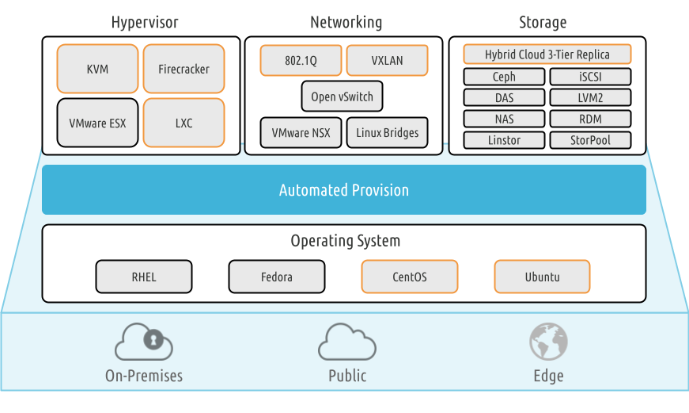
\includegraphics[scale=0.6]{Images/Open_Nebula.png}
    \caption{Open Nebula's architecture}
\end{figure}
\subsection{OpenStack}
OpenStack is a cloud solution originally developed by NASA, it provides a cloud operating system that can control large pools of compute, storage and networking resources. A dashboard is also available. \n
OpenStack goes beyond standard IaaS functionally, it provides additional components, orchestration, fault management and service management amongst other services to ensure high availability of user applications. The following is the architecture of OpenStack.
\begin{figure}
    \centering
    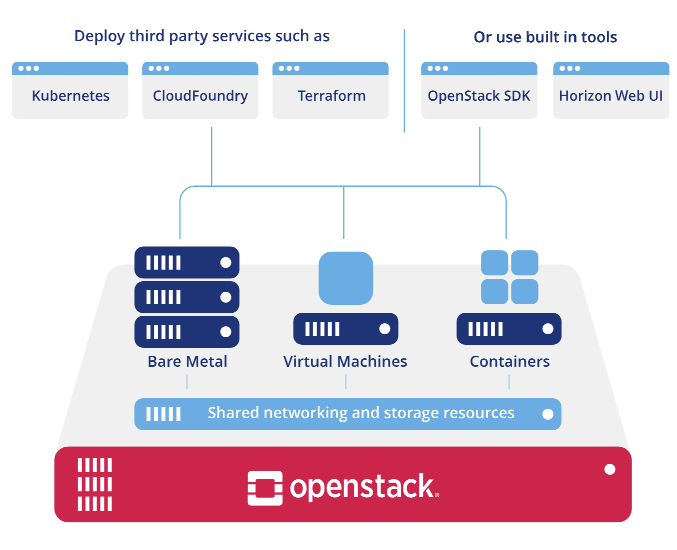
\includegraphics[scale=0.6]{Images/OpenStack.png}
    \caption{OpenStack's architecture}
\end{figure}
OpenStack's dashboard implements a GUI to retrieve, acess and automatize cloud resources, it permits the delivery of third party services like billing and monitoring. It provides an overview on the cloud dimension and status and permits to create users and projects, assigning users to projects and limit the use of resources. OpenStack provides a flexible architecture developed for horizontal scaling. \n
When it comes to storage OpenStack supports both Object Storage and Block Storage:
\begin{itemize}
    \item Object storage provides storage with optimized costs and ability to scale out, it's nbot a traditional file system because it stores data in objects.
    \item Block storage permits to connect block devices to compute instances to achieve greater performance and integrates with enterprise storage platforms.
\end{itemize}
OpenStack's networking is scalable, based on APIs and is pluggable, which means that users can create their own network, control traffic and connect servers and devices. \n
The following is a diagram of the various OpenStack services.
\begin{figure}
    \centering
    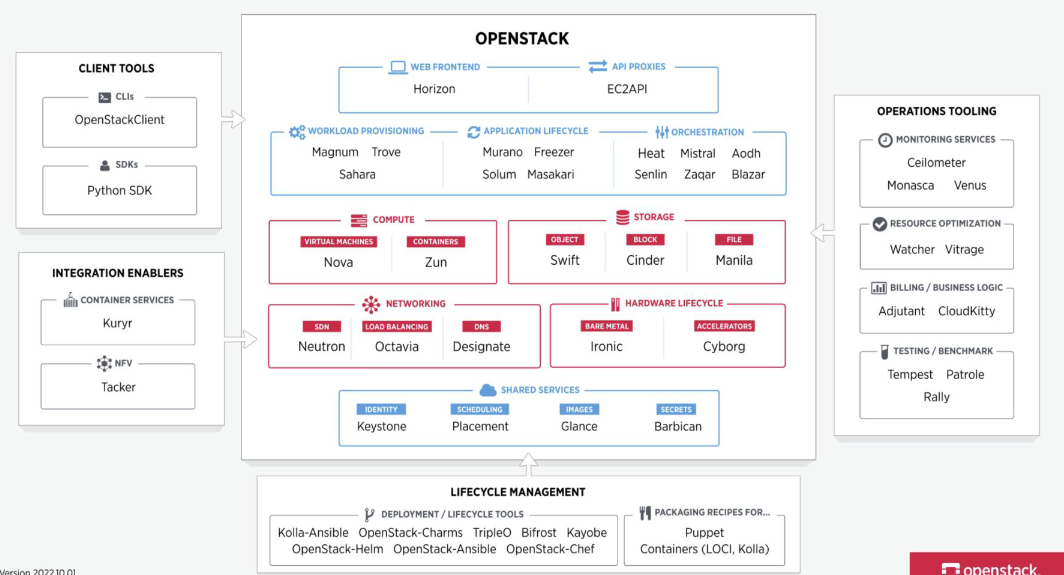
\includegraphics[scale=0.4]{Images/OpenStack_Services.png}
    \caption{OpenStack services}
\end{figure}
OpenStack's dashboard, \textbf{Horizon}, is based on Django and can be accessed by clients and APIs od any OpenStack services. Admin endpoints provide admin functionalities through the dashboard. \n
\textbf{Nova} is a fundamental service of OpenStack infrastructure, it manages the entire lifecycle of the VM instances in the virtualized environment. It handles horizontal scalability on standard hardware and can retrieve images needed for instance creation. Nova-network daemon is used for network management. \n
\textbf{Neutron} is a networking service that allows the creation and implementation in the virtual network of devices and interfaces managed by other OpenStack services. It interacts with the compute service to provide a network infrastructure and support network access to the instances. \n
The main operations are port plugging and unplugging, net and subnet creation and IP addressing. Plug-in agenst differ on the basis of the provider and technologies ursed to implement the cloud environment. Nova-network and Neutron are two different implementations of the Networking-as-a-Service (NaaS) paradigm for OpenStack. \n
\textbf{Cinder} adds persistent storage to a VM, the data is maintained until the VM is canceled and provides an infrastructure to manage volumes and volume snapshots. \n
\textbf{Swift} is a multi-tenant object storage system, it's used to store data and images of VMs, data is maintained until the VM is cancelled and can be accessed everywhere. It provides abstractions to store methods, not storage itself. \n
\textbf{Keystone} has two main functions, it tracks users and corresponding privileges, it provides a list of services available with API endpoint. Keystone generates authorization tokens for users.
\textbf{Glance} is the image manager, it accepts requests for disk images or server images, VMs, or metadata corresponding to images of end users or OpenStack compute components. \n
It supports provisioning from different types of repositories. \n
\textbf{Ceilometer} is the telemetry manager, it collects data from OpenStack services regarding different components of the infrastructure. It can send alarms when collected data violates predefined rules and contains:
\begin{itemize}
    \item Compute-agent
    \item Central-agent
    \item Notification-agent
    \item Collector
    \item Alarm evaluator
    \item Alarm notifier
    \item API server
\end{itemize}
\textbf{Heat} is the orchestration manager providing a template-based orchestration. Allows automation of the infrastructure deplyment. The template language allows to:
\begin{itemize}
    \item Specify virtual machine configurations (compute, storage and network)
    \item Specify post-deployment activities
    \item Create many types of OpenStack resources
\end{itemize}
Heat allows developers to directly integrate the orchestration module via a custom plug-in. \n
OpenStack contains four different networks:
\begin{itemize}
    \item Management network
    \item Data network
    \item External network
    \item API network
\end{itemize}
The way they interact with the OpenStack system is summarized in figure 10.
\begin{figure}
    \centering
    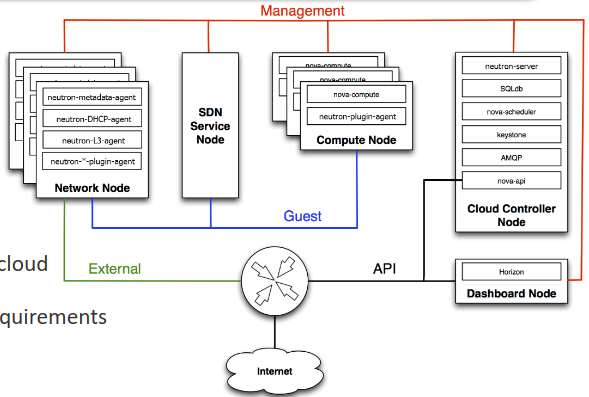
\includegraphics[scale=0.5]{Images/OpenStack_network.png}
    \caption{The OpenStack networks}
\end{figure}
\section{PaaS}
\section{Data Governance and Management}
As we have said countless times up to this point, cloud computing is a very complex matter, the NIST definition can be found back in section 5.4 and the issues of the model are the following:
\begin{itemize}
    \item (Micro)Services composition
    \item Untrustworthy data
    \item High dynamics and flexibility
    \item Multi-domain evaluation
\end{itemize}
The natural evolution of cloud spanning an even bigger area is IoT, IoT is \textit{The intelligent connectivity of physical devices driving massive gains in efficency, business growth and quality of life}. \n
The first big step in that direction was made with 5G, high-speed connectivity with very low latency is one of the basic requirements to start setting up the needed infrastructure for a smart city. \n
In an IoT setting the cloud will have a layered and hierarchical structure with cloud data centers, that exchange informations with fog nodes that pre-process data coming from the edge of the cloud which are all the cameras and sensors embedded in smart systems. Having many sensors connected and collecting data every minute requires a very good metrics and analytics system to process the data coming from the edge and implement specific management functionalities. \n
It's obvious that the time has come to talk a bit about big data and more data driven techniques. \n
The 5 Vs of big data are the following:
\begin{itemize}
    \item Volume, the size of the data
    \item Velocity, the speed at which the data is generated
    \item Variety, the different types of data
    \item Veracity, The trustworthiness of the data in terms of accuracy
    \item Value, having data is of no use unless they can be turned into value
\end{itemize}
The data analytics pipeline is shown in figure 12
\begin{figure}
    \centering
    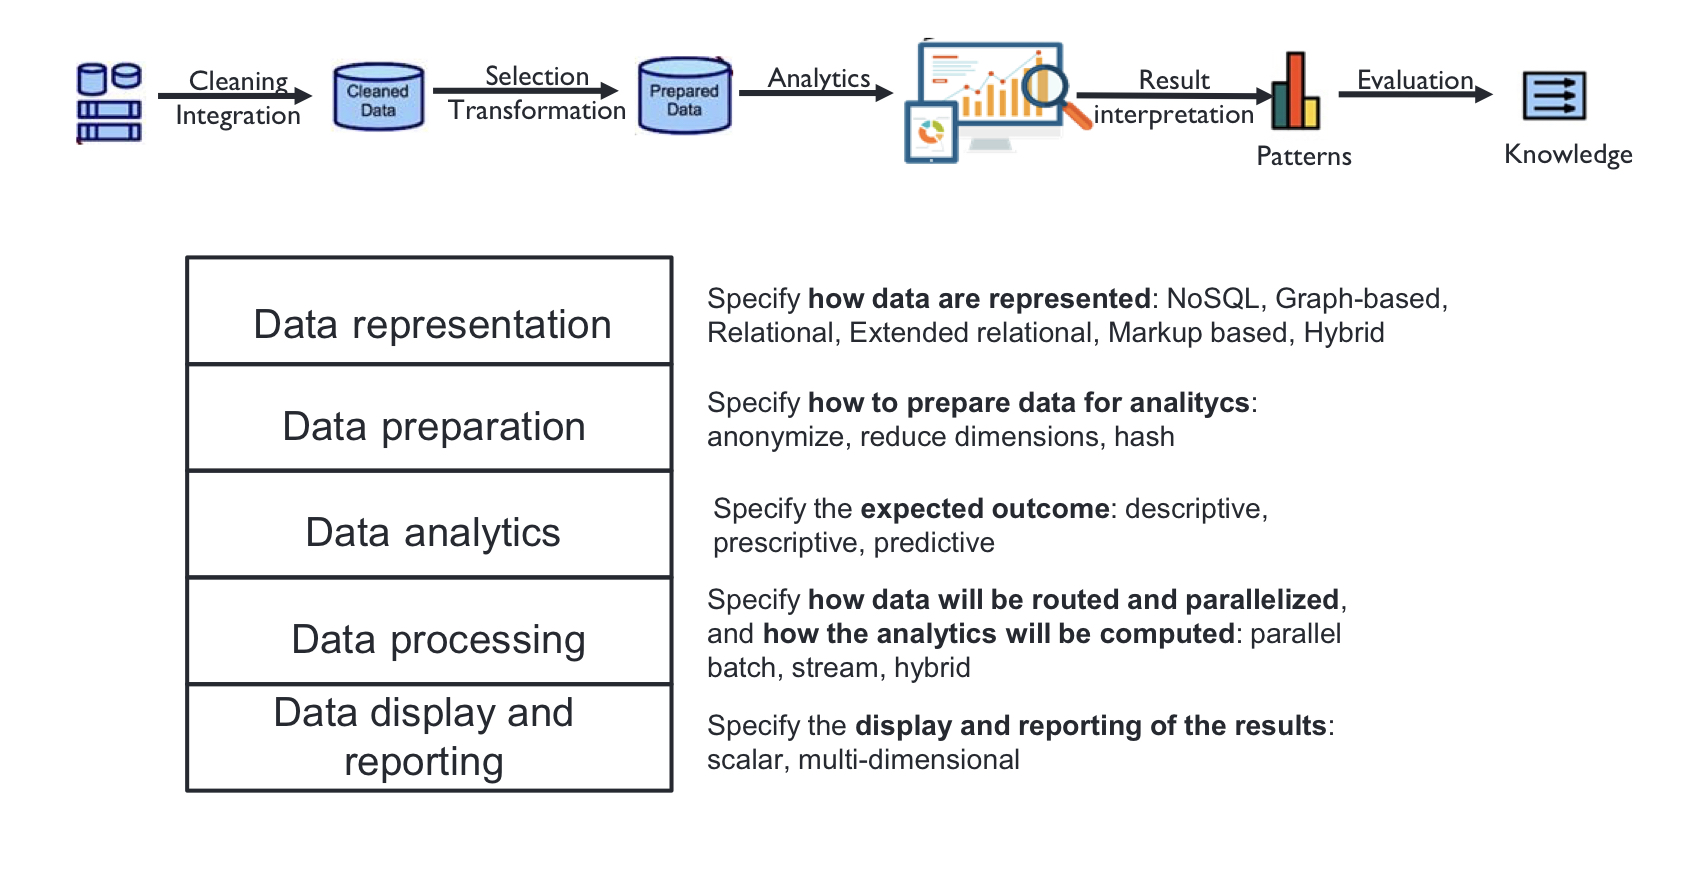
\includegraphics[scale=0.2]{Images/data_analytics_pipeline.jpeg}
    \caption{The data analytics pipeline}
\end{figure}
Since companies have seen how profitable can be a data-driven development process big data technologies have grown tremendousl in the past few years but there has been an incredible shortage of data scientists and data engineers, the demand is far from being met. \n
Only 30\% of businesses have a fully integrated data-analytics pipeline, 38\% of the businesses are struggling even with proofs of concept, key challenges associated with the development and management of Big Data initiatives are:
\begin{itemize}
    \item Lack of skills and clarity on Big Data technology (many people in the business do not even know that in data there is money to be made)
    \item Lack of general architecture and lack of standard processes
    \item Ineffective governance models
\end{itemize}
The biggest implementation challenges today in the field of Big Data are that: it's really hard to store and manage data in different places and formats, plus there is no coordintation in the field of big data / AI initiatives, solving the problem of handling massive amounts of data is not trivial both from an implementation and an engineering stand point, dated data and inability to operationalize insights and big data tool selection. \n
Getting into big data at this point in time can be done with many open source alternatives when it comes to both big data processing frameworks, storage and implementation languages. The incredible amount of alternatives allows companies to choose whichever technological stack they prefer without having to bind to one specific producer. \n
As I said, thanks to the power of alternatives, there are a bunch of commercial analytics platforms that are built on top of big data open source technologies (Apache Hadoop, Spark, Storm, etc...) the leaders in this space are Cloudera, Hortonworks and IBM insights, this is a summary of their features:
\begin{itemize}
    \item Provide enterprise-ready Hadoop distributions
    \item Management of Hadoop clusters
    \item Performance analytics
    \item Security and SLA monitoring
    \item Support for integrated marketing solutions
\end{itemize}
When it comes to data governance most technologies also offer data preparation functionalities like: ETL or ELT (Extract, Transform and Load). \n
Data storage and preparation tools offer:
\begin{itemize}
    \item Data inventory
    \item Metadata management
    \item Data quality
    \item Data integration
    \item Data security
    \item Fault tolerance
    \item ELT, ETL
    \item SLA monitoring
\end{itemize}
There are many providers when it comes to analytics and visualization technology. A summary of the offered features is:
\begin{itemize}
    \item Graphical interface to design analytics model
    \item Store the analysis result to different databases
    \item Provide data training and validation environment
\end{itemize}
Up to this moment we have basically reinforced the fact that there is a plethora of different big data technologies to choose from, picking a stack that suits the needs of the client can be a very complex task, it's important to keep in mind the fact that there is no single big data technology and balance between bottom-up and top-down approaches should be found. An example of the selection process is shown in figure 13.
\begin{figure}
    \centering
    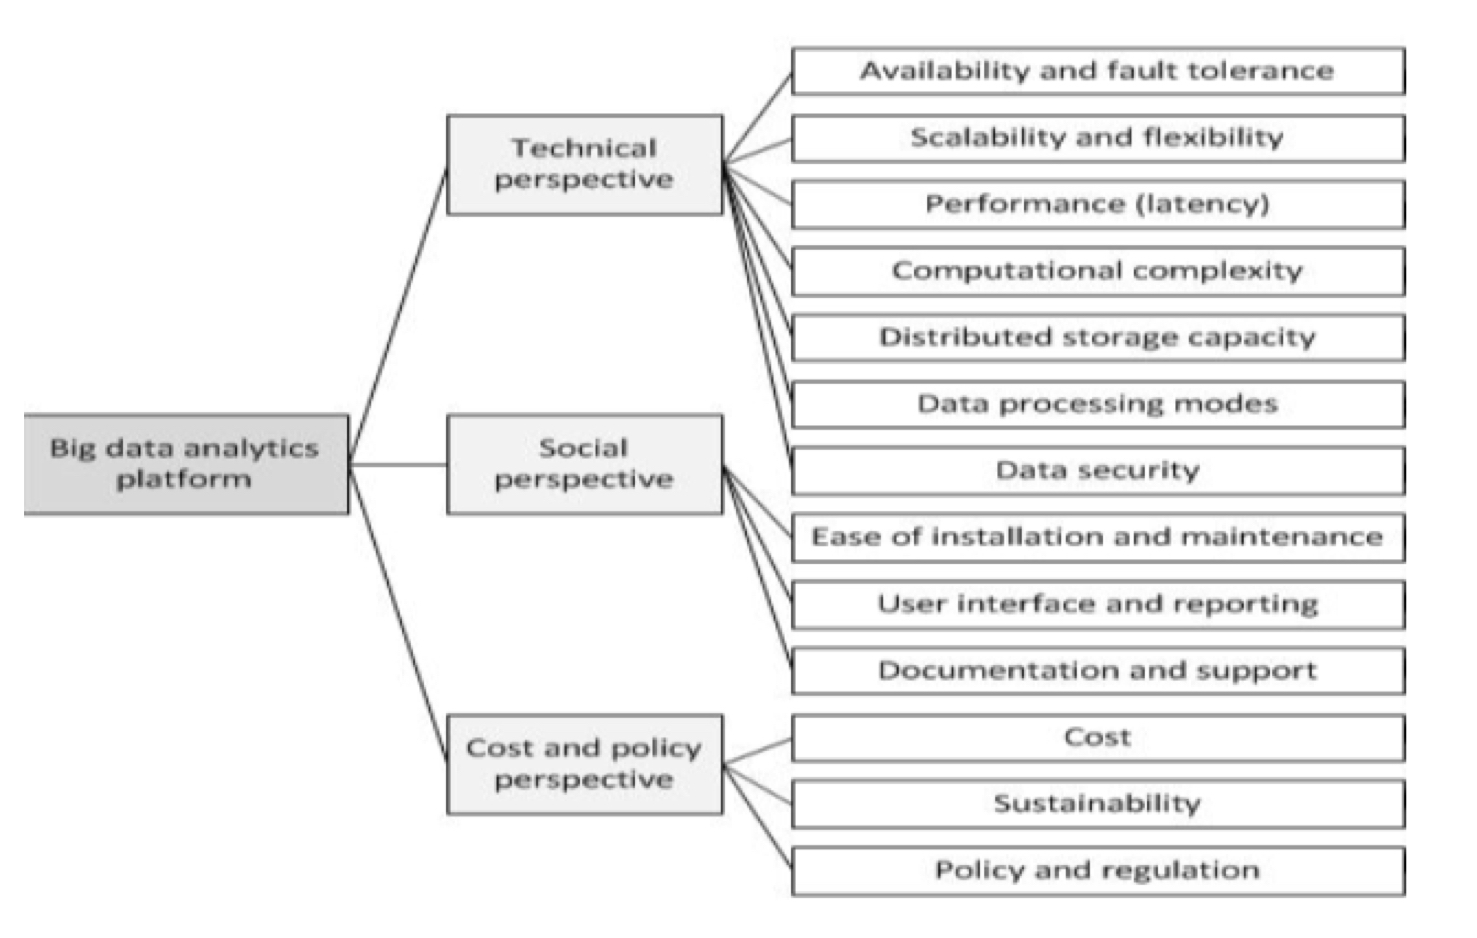
\includegraphics[scale=0.2]{Images/tech_selection_process.jpeg}
    \caption{Example of criterion to select big data technologies}
\end{figure}
\subsection{Big Data as a Service (BDaaS)}
We have said that entering the world of big data is a hustle, we have also said that there are not enough people to meet the work demand in the field and that there is a heck of a lot of money to be made from the good use of users data. \n
Point is? \n
A new company wanting to enter the scene (not necessarily in the tech world) and needing a big data system gets to a point where they find themselves in a situation where they have options, too many options, and no easy solution to all the mess. \n
Somebody thought it would be really cool to merge cloud business logic with big data. What if, I gave you a ready to use infrastructure, no further knowledge required, to handle your big data needs, in exchange for a fee? No need to lose your wits on a big data infrastructure implementation, that's for sure. \n
BSaaS are not just about storage and cost, these solutions offer built-in systems for artificial intelligence and analytics, you can accomplish some pretty impressive results without having to have a huge team of data analysts, scientists and architects around you. \n
The advantages of BDaaS are pretty obvious:
\begin{itemize}
    \item Makes managing big data easier
    \item Opens up big data for a range of medium-sized businesses
    \item It's a very low cost solution compared to the alternative of running your own metal (just like with the clud)
\end{itemize}
There are three different BDaaS models:
\begin{itemize}
    \item Big data infrastructure as a service, it's a IaaS offer including basic data services from a cloud serivce provider.
    \item Big data platform as a service, is a PaaS offer for an all-round big data stack.
    \item Big data software as a service, a SaaS offer which is self contained in a single tool.
\end{itemize}
How does the big data IaaS model work? There is a data layer, consisting of either: Hadoop, NoSequel databases and Relational databases; a compute layer, which can either be: Self-built ETL scripts, Commercial ETL tools or open source processing tools. \n
If we climb the stack a PaaS model can be (if we consider Amazon's implementation) a standard Hadoop implementation with:
\begin{itemize}
    \item Data ingestion, logs file data from any data source
    \item Amazon S3 data storage layer
    \item Analytics and visualization
\end{itemize}
A similar setup is implemented by competitors. \n
Last but not least, getting to the SaaS level, a fully hosted big data stack that includes everything from data storage to data visualization has the following:
\begin{itemize}
    \item Data layer
    \item Integration layer, pulls the data out of the database and into a flexible modeling layer
    \item Processing layer
    \item Analytics and BI layer
\end{itemize}
The differences between the various models can be summarized as follows:
\begin{itemize}
    \item IaaS is way more expensive than the other two models but allows almost complete control over resources and allows a custom implementation of complex data pipelines. It is not an easy thing to handle and is an hardcore alternative.
    \item PaaS is a much easier thing to master, it allows for a decent level of customization and control but it also requires a good level of expertise to handle compared to SaaS options.
    \item SaaS is a very low cost solution which is not that customizable but can tick many boxes for low to medium sized companies.
\end{itemize}
\subsection{Apache pipeline}
The Apache pipeline is shown in Figure 14 and includes the Hadoop framework, which is designed to store and process large amounts of data on clusters made of commodity hardware. It constitutes the lowest layer of the architecture and provides storage and resource management. \n
It also provides the Map Reduce processing model that allows concurrent scanning of multiple files, the model does not suffer from data intensive activities. \n
Hadoop is a distributed filesystem written in Java, based on the concept of distributing blocks across a series of different nodes. Hive is a structured data warehouse based on Hadoop capable of managing large datasets that reside in distributed storage.
\begin{figure}
    \centering
    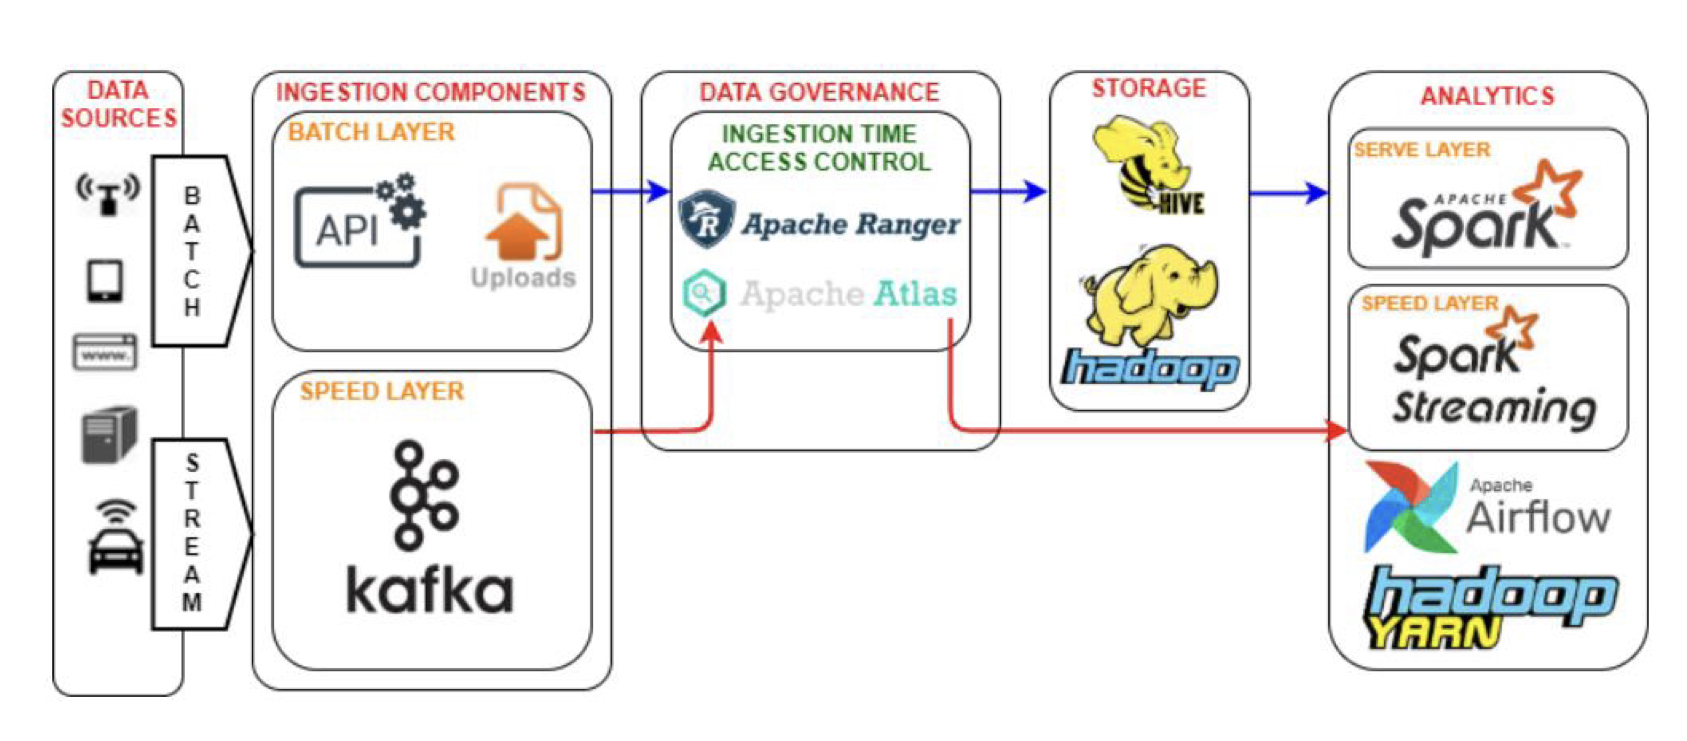
\includegraphics[scale=0.2]{Images/apache_architecture.jpeg}
    \caption{The Apache data pipeline}
\end{figure}
For the analytics section there is:
\begin{itemize}
    \item Hadoop YARN, which is the resource manager of the Hadoop cluster.
    \item Apache Spark, which is an analytics engine for large scale data processing, along with it there is Spark streaming that allows for large-scale stream (Kafka does stream ingestion) processing.
    \item Apache Airflow i an orchestrator of processing pipelines aimed at providing scheduling and monitoring capabilities.
\end{itemize}
Batch ingestion is handled via common APIs (like REST).
\subsection{Enterprise Data governance}
I think that I've skipped on the concept for a long while, what is Data Governance?
According to wikipedia: \textit{data governance is a data management concept concerning the capability that enables an organization to ensure that high data quality exists throughout the complete lifecycle of the data, and data controls are implemented that support business objectives}. \n
In the world of enterprise the point is to provide a common approach to data governance across all systems and data within the organization. An enterprise data governance should be:
\begin{itemize}
    \item Transparent - governance standards and protocols must be clearly defined and available to all.
    \item Reproducible - recreate the relevant data landscape at a point in time should be possible.
    \item Aubditable - all relevant events and assets must be traceable with appropriate historical lineage.
    \item Consistent - compliance practices must be consistent.
\end{itemize}
If we get back to the example of the Apache sute, two components play fundamental role for data governance:
Ranger (which is a policy editor and handles access control) and Atlas (which handles fine-grained data control via tagging). \n
\subsubsection{Apache Ranger}
Ranger gives centralized authorization and auditing across Hadoop components, it has an extensible architecture with custom policy conditions, context enrichers and more. \n
Policies are rules that decide how and who can access specific sets of resources and resource classifications. There are different policy types:
\begin{itemize}
    \item Access authorization based on resources or resource classification
    \item Row filter, column-masking based on policies, that can be done by restricting the rows accessible in a table based on users/groups/runtime-context or by masking/anonimizing sensitive columns.
\end{itemize}
\begin{figure}
    \centering
    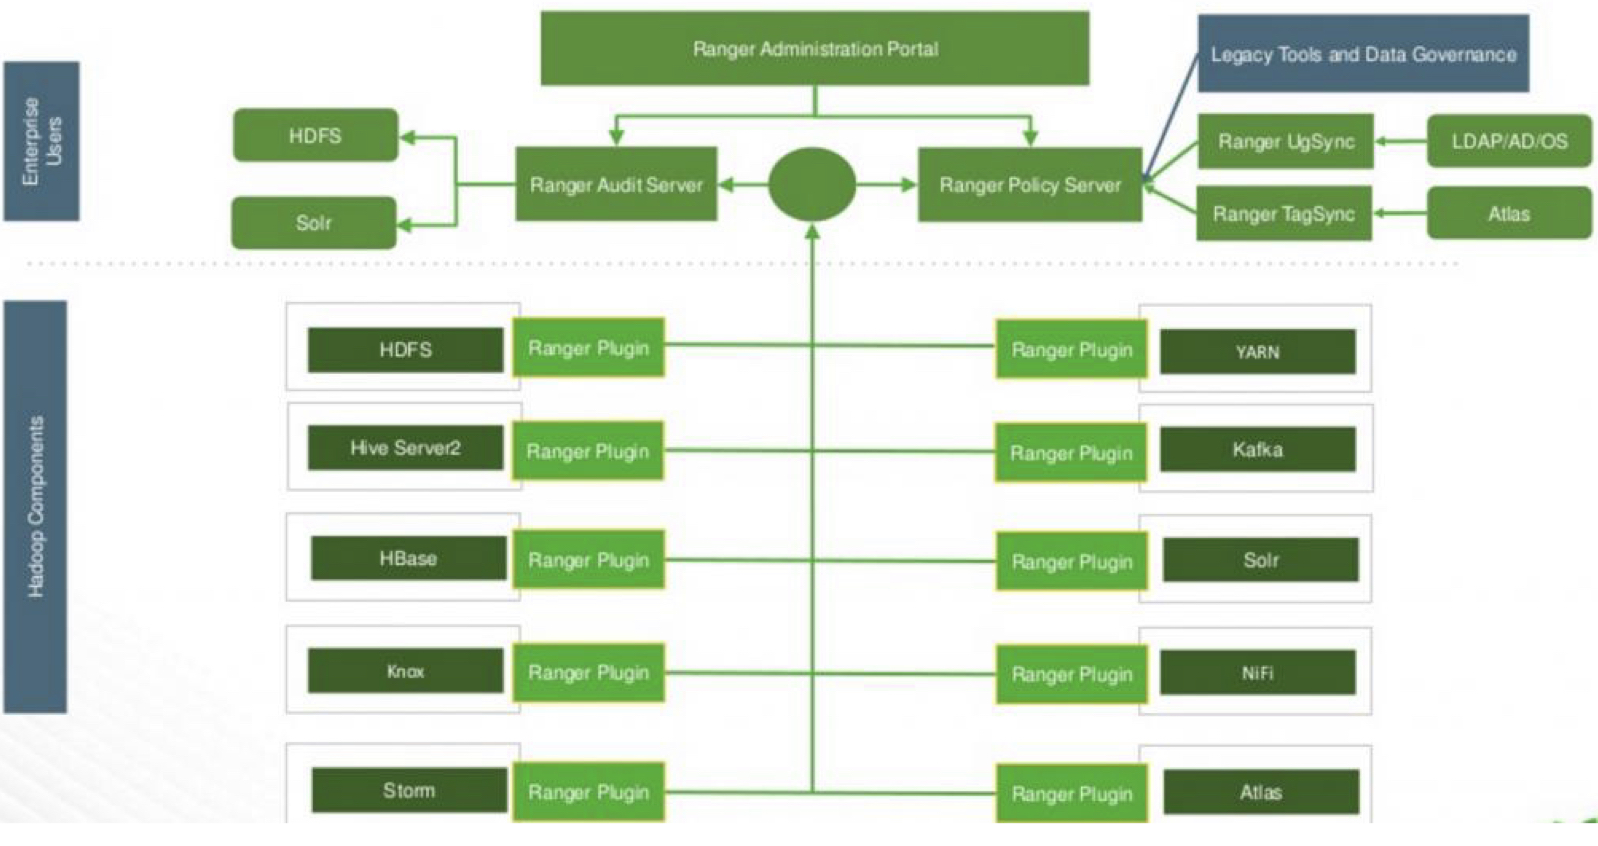
\includegraphics[scale=0.2]{Images/Ranger_architecture.jpeg}
    \caption{Ranger architecture}
\end{figure}
Ranger's architecture is shown in Figure 15. \n
The tags used in Ranger are created in Atlas and can be attatched to metadata, which can be a column, a table, an HDFS path, etc\dots \n
Plugin of each service saves tags info into policy and can be cached locally for fast retrieval. The flow of evaluation for tag policies is shown in Fiugre 16.
\begin{figure}
    \centering
    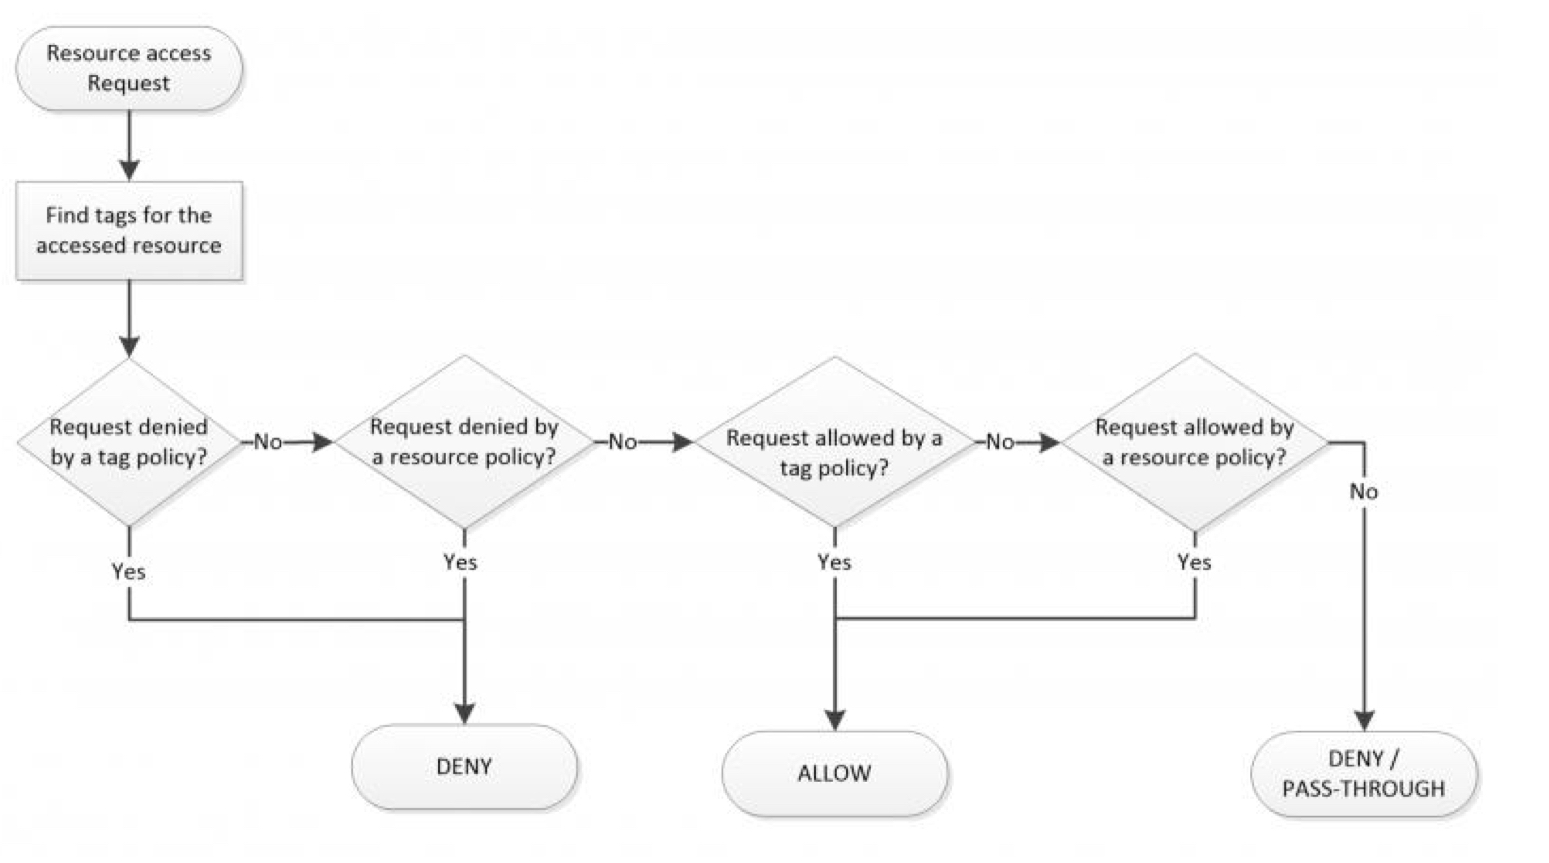
\includegraphics[scale=0.2]{Images/policies_evaluation.jpeg}
    \caption{The policies evaluation pipeline}
\end{figure}
\subsubsection{Apache Atlas}
Atlas provides open metadata management and governance capabilities for organizations to build a catalog of their data assets, classify and govern these assets and provide collaboration capabilities around these data assets for data scientists, analysts and the data governance team. \n
Atlas also provides:
\begin{itemize}
    \item Lineage
    \item Search/Discovery
    \item Support for Apache Ranger Security and Data Masking
\end{itemize}
Atlas keeps in memory a metadata repository with a flexible type system to capture schema/metadata of multiple components. \n
Is, obviously, perfectly integrated with Apache Hive, Storm, Falcon, Sqoop for metadata and lineage and also with Ranger for classification-based security. \n
It also provides APIs to support for more components. \n
\subsection{Data ingestion procedure}
\etl and \elt are two different ways of doing data ingestion and manipulation, the basic difference is that they are doing the same operations in a different fashion. \n
The basic operations are the following:
\begin{itemize}
    \item Extract - extraction refers to pulling the source data from the original database or data source. \etl puts data into a temporary staging area, while \elt sends data immediately into a data lake storage system.
    \item Transform - Transformation refers to the process of changing the structure of information, so it integrates with the target data system and the rest of the data in that system.
    \item Loading refers to the process of depositing the information into a data storage system.
\end{itemize}
\subsubsection{\etl}
\etl is typically used in data warehouses, the advantages of \etl are:
\begin{itemize}
    \item Pre structured nature of the OLAP (OnLine Analytical Processing) data warehouse
    \item Compliance to various laws like GDPR, HIPAA or CPAA.
    \item \etl was born over two decades ago and has been used a lot.
\end{itemize}
\subsubsection{\etl}
The \etl process also works with data lakes, a data lake is a special kind of data store accepting any kind of structured or unstructured data, there is no need to transform data before loading it. \n


\end{document}